\subsection{Opsamling af accelerometer-signaler}\label{sec:acc_imp}

I dette projekt anvendes der på baggrund af krav opstillet i \autoref{sec:acc_teori} to accelerometre ADXL335Z fra Analog Devices. Accelerometerne er en 3-aksialt sensor, som har et arbejdsområde på minimum $\pm3~g$, og en spænding som output. Det analoge outputsignal er proportionalt med accelerationen \citep{analogdevices2009}. 

Accelerometrene har en single-supply spændingsforsyning, som skal ligge mellem $1,8~-~3,6~V$.  Offsettet er afhængig af forsyningsspændingen fra mikrokontrolleren, der forsyner accelerometrene. Forsyningsspændingen er $3,3~V$, og derved bliver offsettet $1,65~V$, som er det halve af forsyningsspændingen. Båndbredden og støjen varierer for akserne. For y-aksen ligger båndbredden mellem $0,5 - 1.600~Hz$.\fxnote{Den spektrale effekttæthed måles i $\mu g/$. Hvis dette divideres med kvadratroden af båndbredden af signalet $\sqrt{Hz}$, fås RMS af accelerationsstøjen ved en temperatur på $25^\circ$C} \citep{analogdevices2010}.

Accelerometrenes outputsensitivitet varierer ligefrem proportionelt med forsyningsspændingen. Sensitiviteten har et range på $\pm10~\%$ \citep{analogdevices2010}. Ved en forsyningsspænding på $3,3~V$ er sensitiviteten $330~mV/g~\pm 10~\%$. 

\begin{figure}[H]
\centering
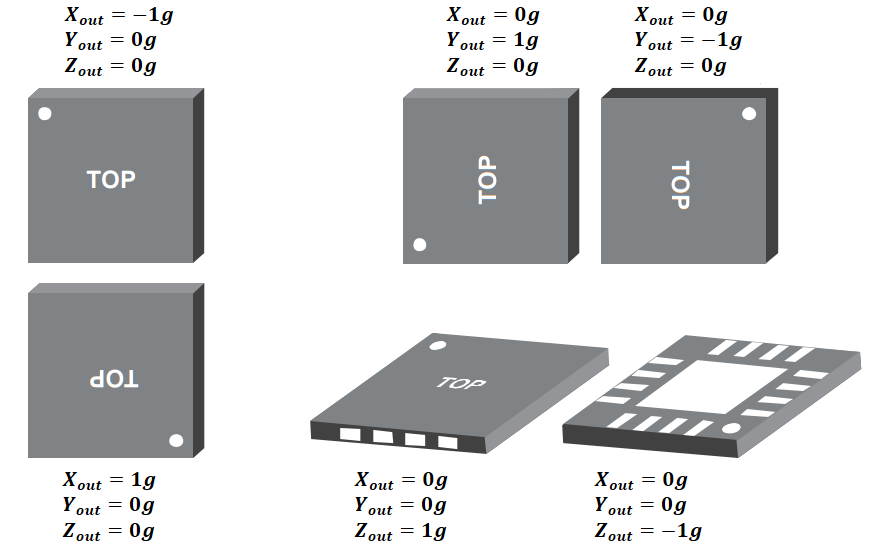
\includegraphics[width=0.85\textwidth]{figures/acc_paavirkning}
\caption{Påvirkning af accelerometeret i forskellige positioner. Til venstre måles accelerometeret lodret, til højre øverst vandret og til højre nederst i plan \citep{analogdevices2010}.}
\label{fig:acc}
\end{figure}

\noindent
Ved hældning af accelerometeret vil der ske en acceleration i forhold til tyngdekraften. Hvilken acceleration, der sker, er afhængigt af plan og hældningens retning. Dette fremgår af \autoref{fig:acc}. Herved vil der ske en ændring i outputspændingen ved en hældning på $0^{\circ}$. Hvis accelerometeret eksempelvis befinder sig i den øverste situation på \autoref{fig:acc}, påvirkes y-aksen med $-1~g$ \citep{clifford2005}. Denne sammenhæng og derved patientens hældning kan udtrykkes ved \autoref{equ:vinkler}, hvor $\phi$ er vinklen i forhold til udgangspunktet for den pågældende akse \citep{clifford2005}.
\begin{equation} \label{equ:vinkler}
	V_{out} = V_{offset} + sensitivitet \cdot \sin(\phi)
\end{equation}